\documentclass[a4paper,pra,twocolumn,10pt,aps,longbibliography,nobalancelastpage]{revtex4-1}


\usepackage{graphicx}
\usepackage{amsmath}
\usepackage{listings}
\usepackage{units}
\usepackage{balance}
\usepackage{float}
\graphicspath{{images/}}



\begin{document}
\title{Real-Time Digital Signal Processing Final Project}
\author{Sagar Patel, CID: 00842688, and Pranav Malhotra, CID: 00823617}
\date{6th March 2017}

\maketitle
\section{Theory}\label{sec:theory} 
For spectral subtraction to be properly implemented, the signal needs to be processed in the frequency domain. The signal is assumed to be corrupted by additive noise and thus its magnitude spectrum is a linear combination of the magnitude spectrum of the original signal and the magnitude spectrum of the noise. \textbf{Although the noise is assumed to be additive, the spectral subtraction methodology does not require the noise to be white. Neither is a priori knowledge of the probability density function (PDF) necessary.}

\begin{figure}[H]
    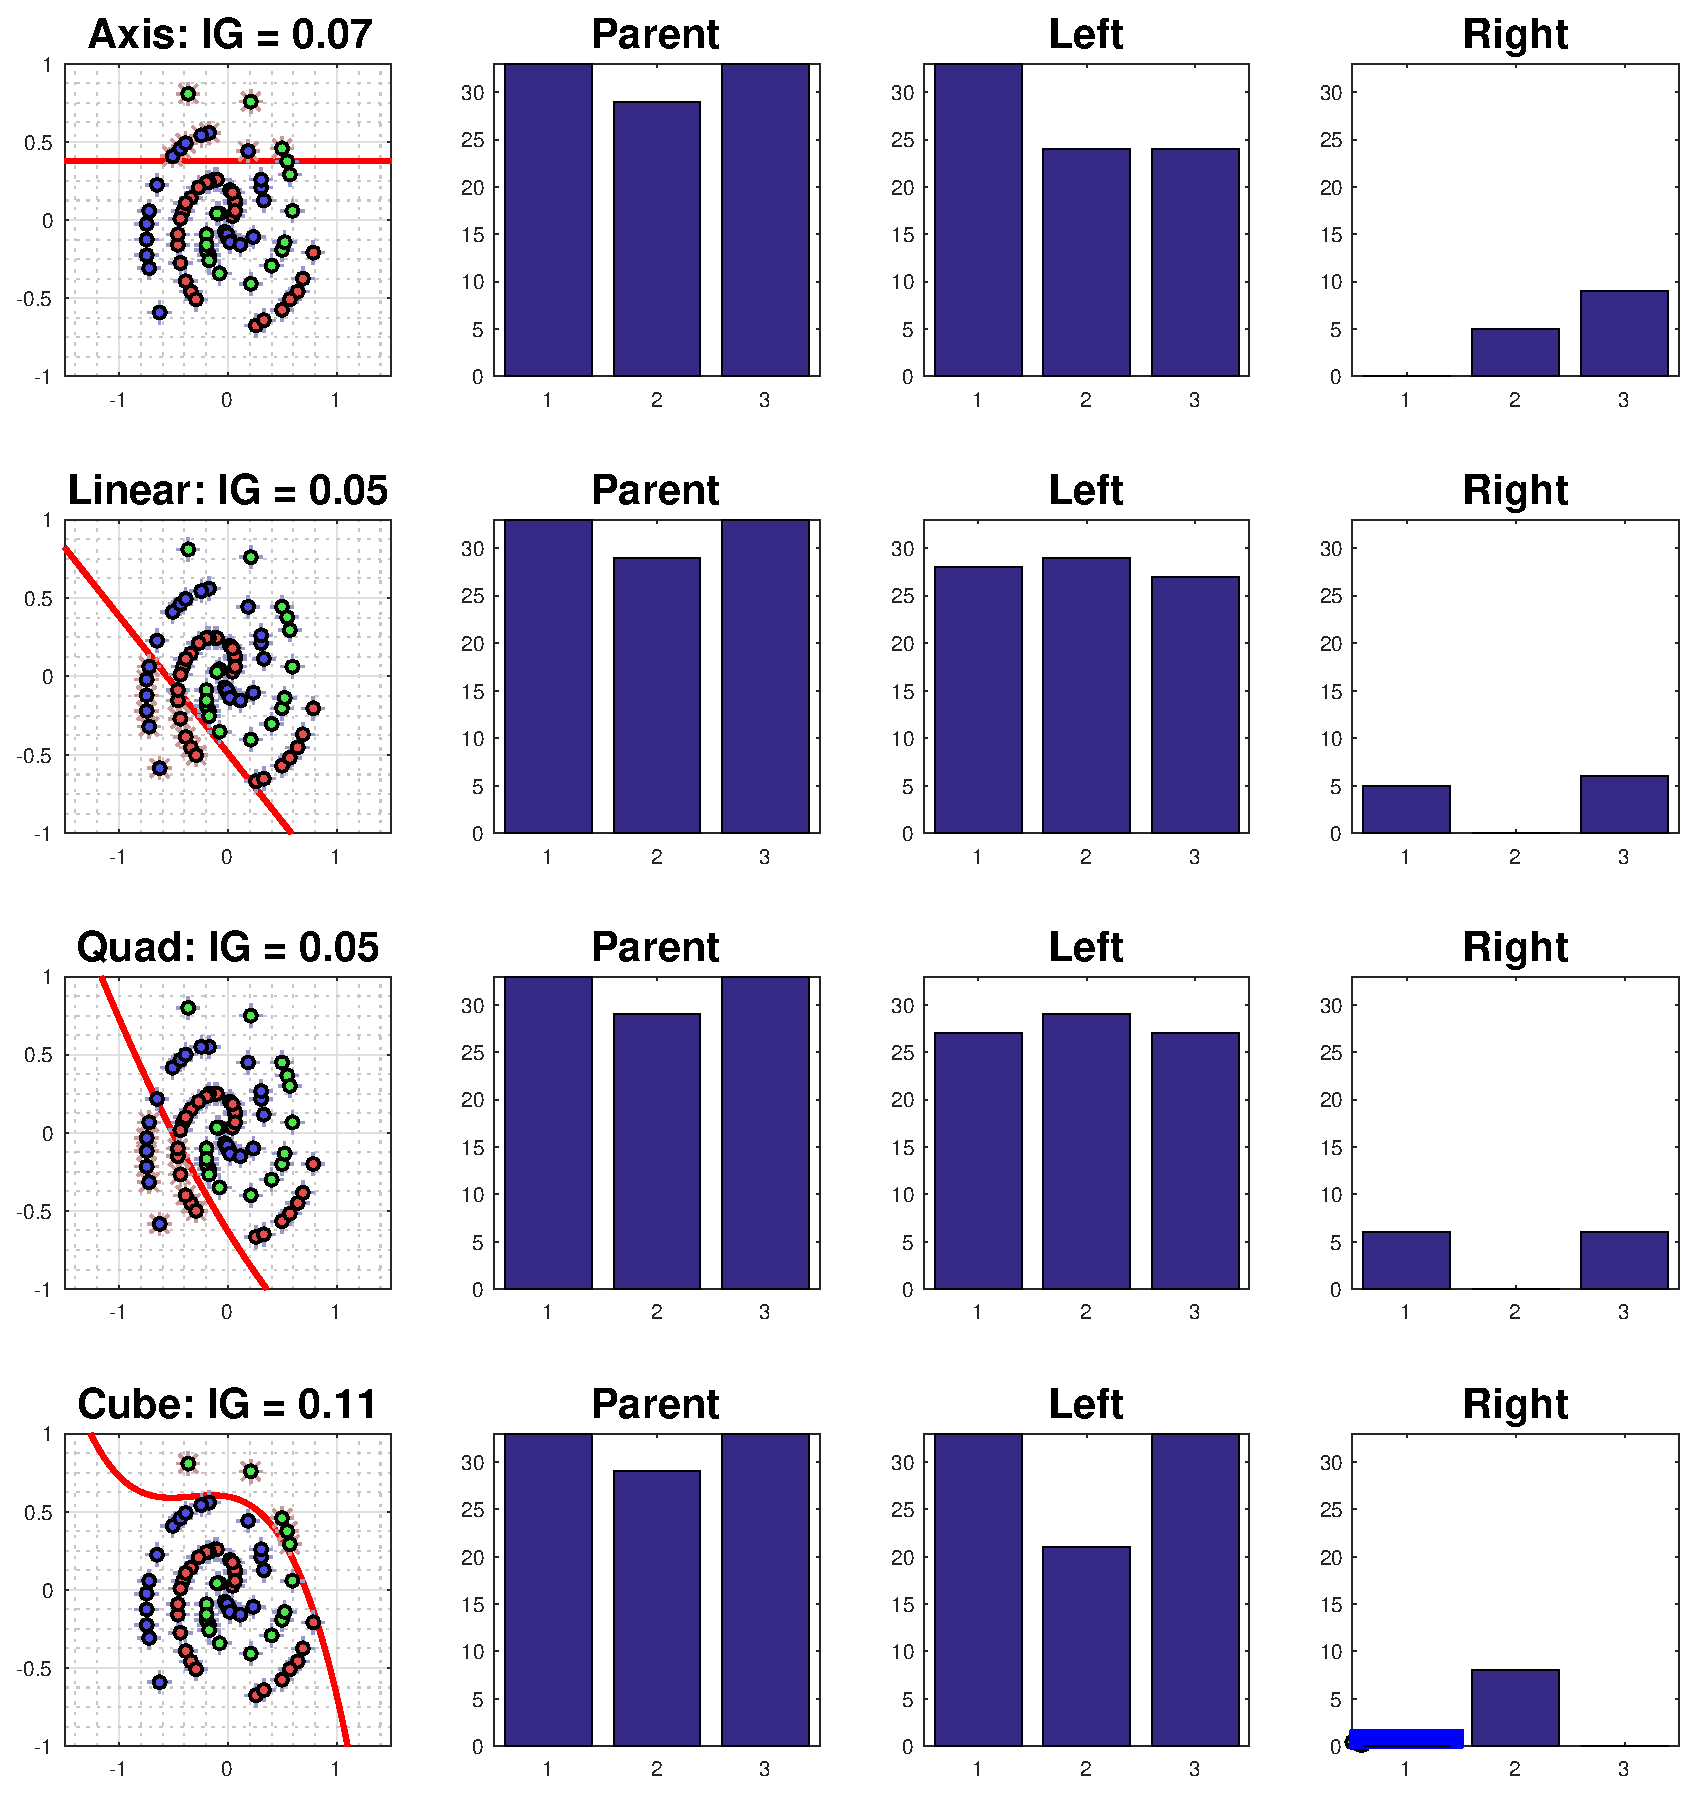
\includegraphics[width=0.49\columnwidth]{split_function_visualitions_1}
    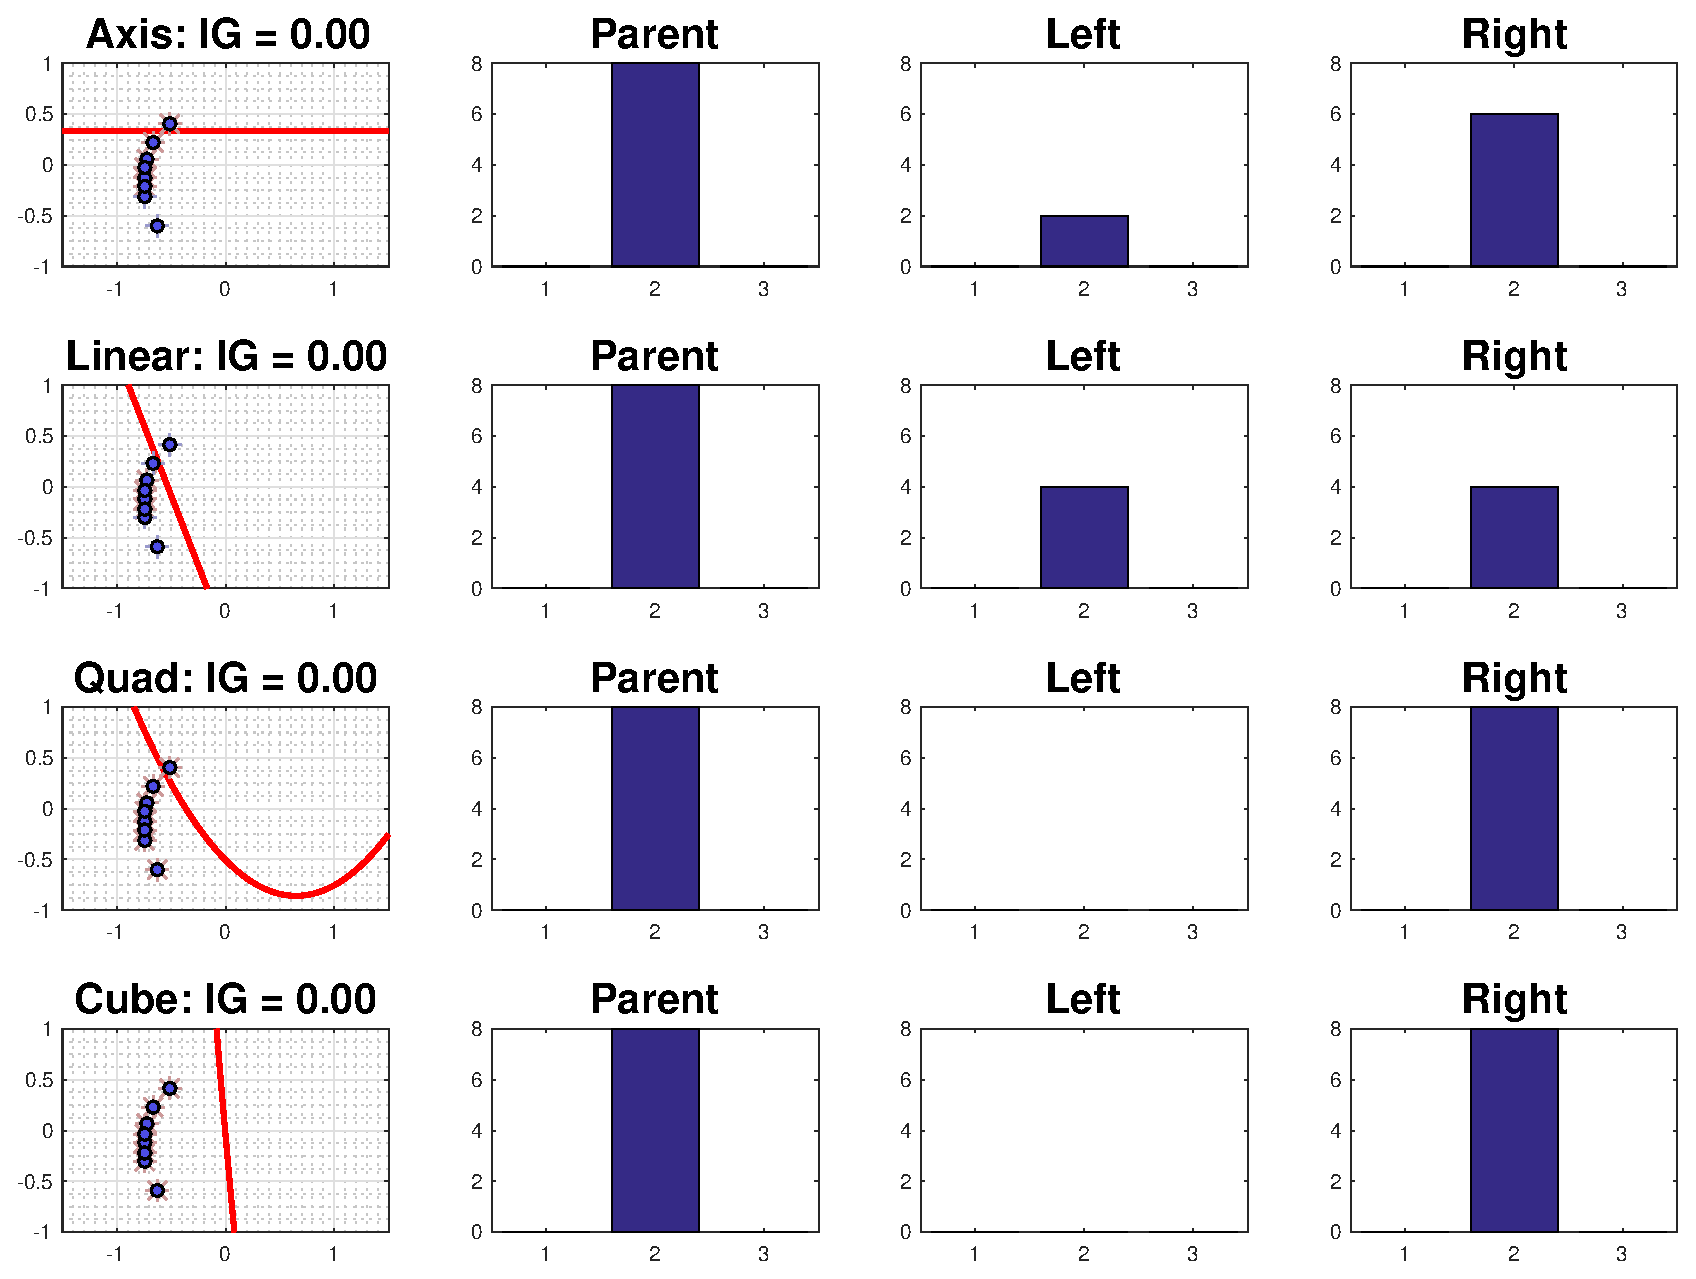
\includegraphics[width=0.49\columnwidth]{split_function_visualitions_2}
    \caption{Overview of spectral subtraction process}
    \label{fig:spec_sub_overview}
\end{figure}

\begin{figure}[H]
    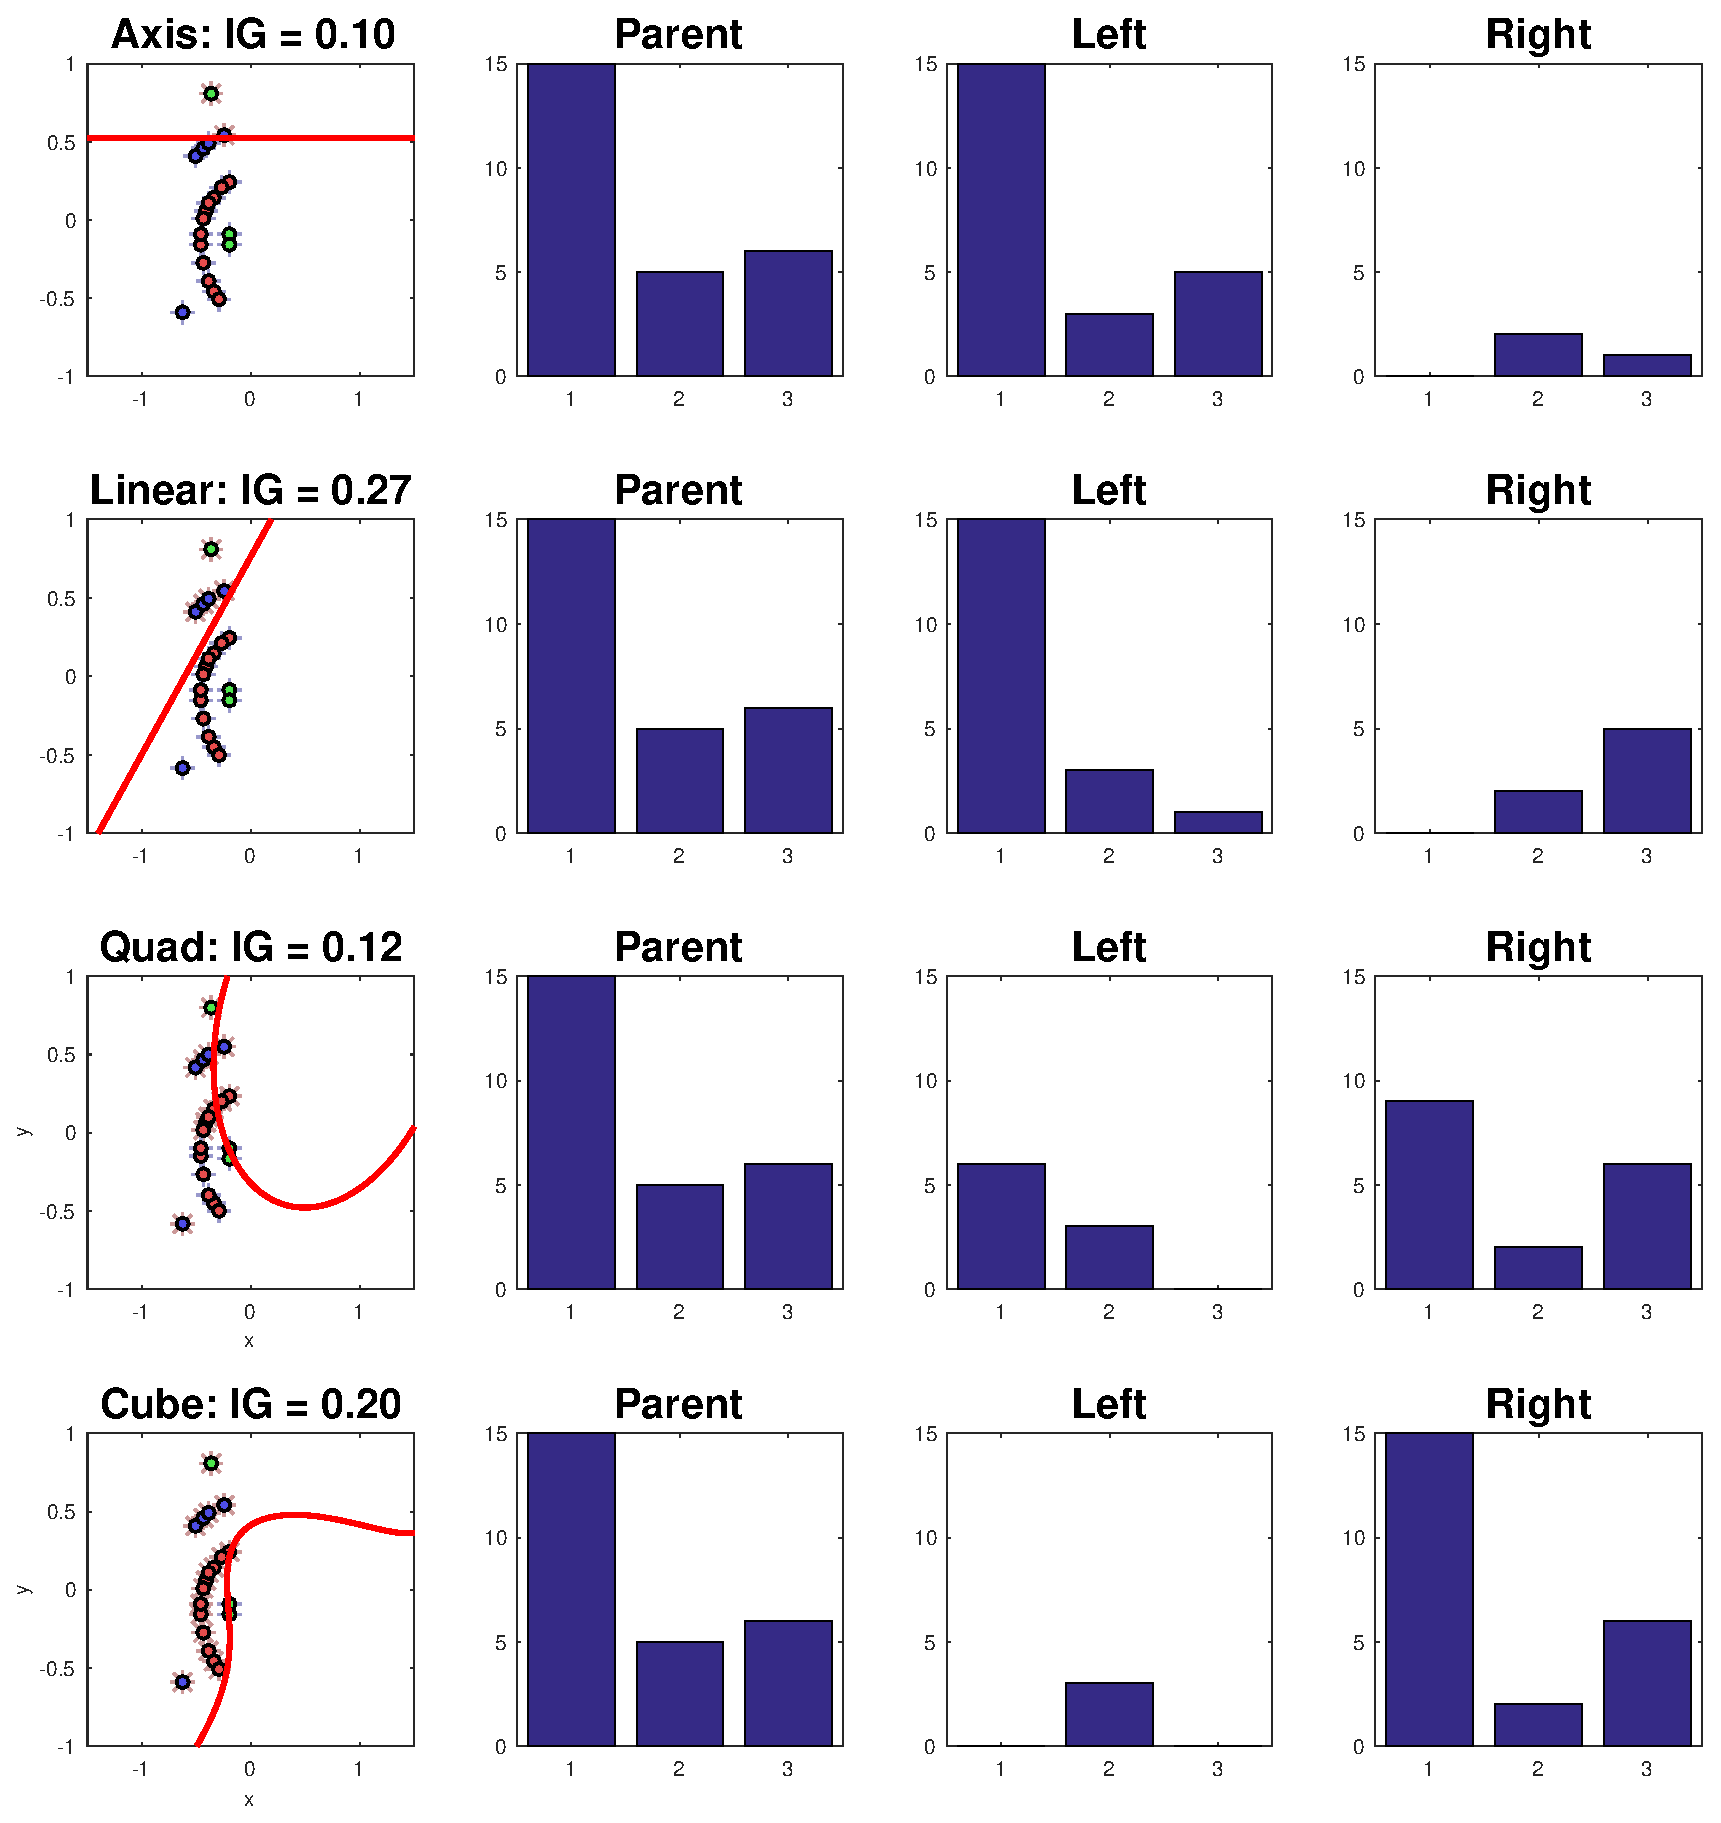
\includegraphics[width=0.49\columnwidth]{split_function_visualitions_3}
    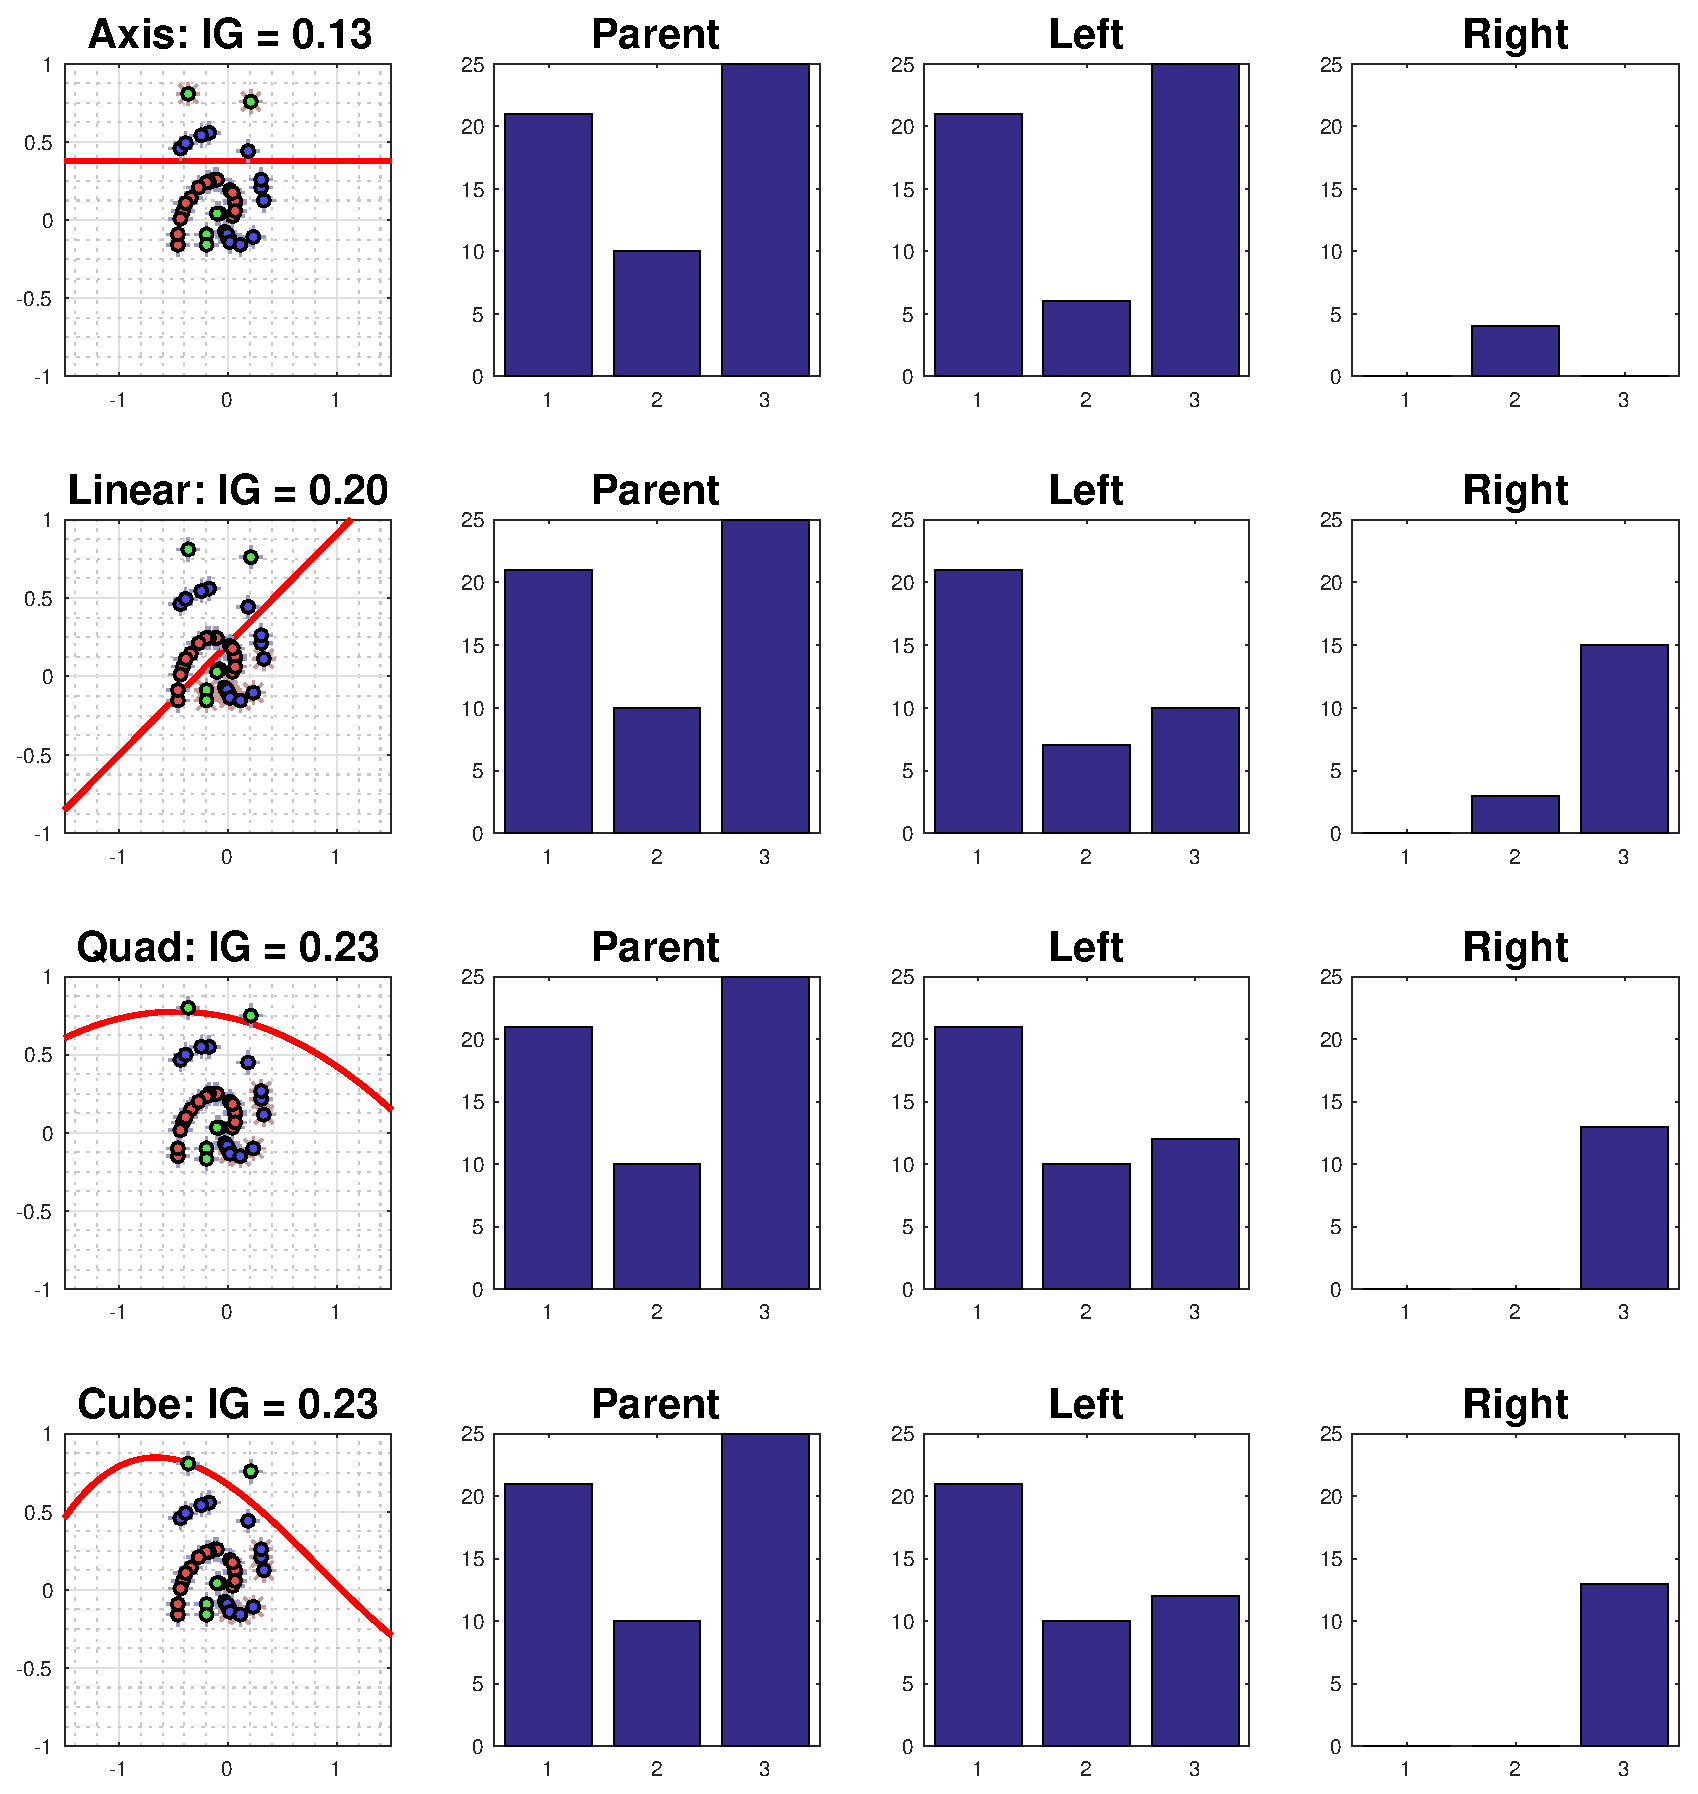
\includegraphics[width=0.49\columnwidth]{split_function_visualitions_4}
    \caption{Overview of spectral subtraction process}
    \label{fig:spec_sub_overview}
\end{figure}

\begin{figure}[H]
    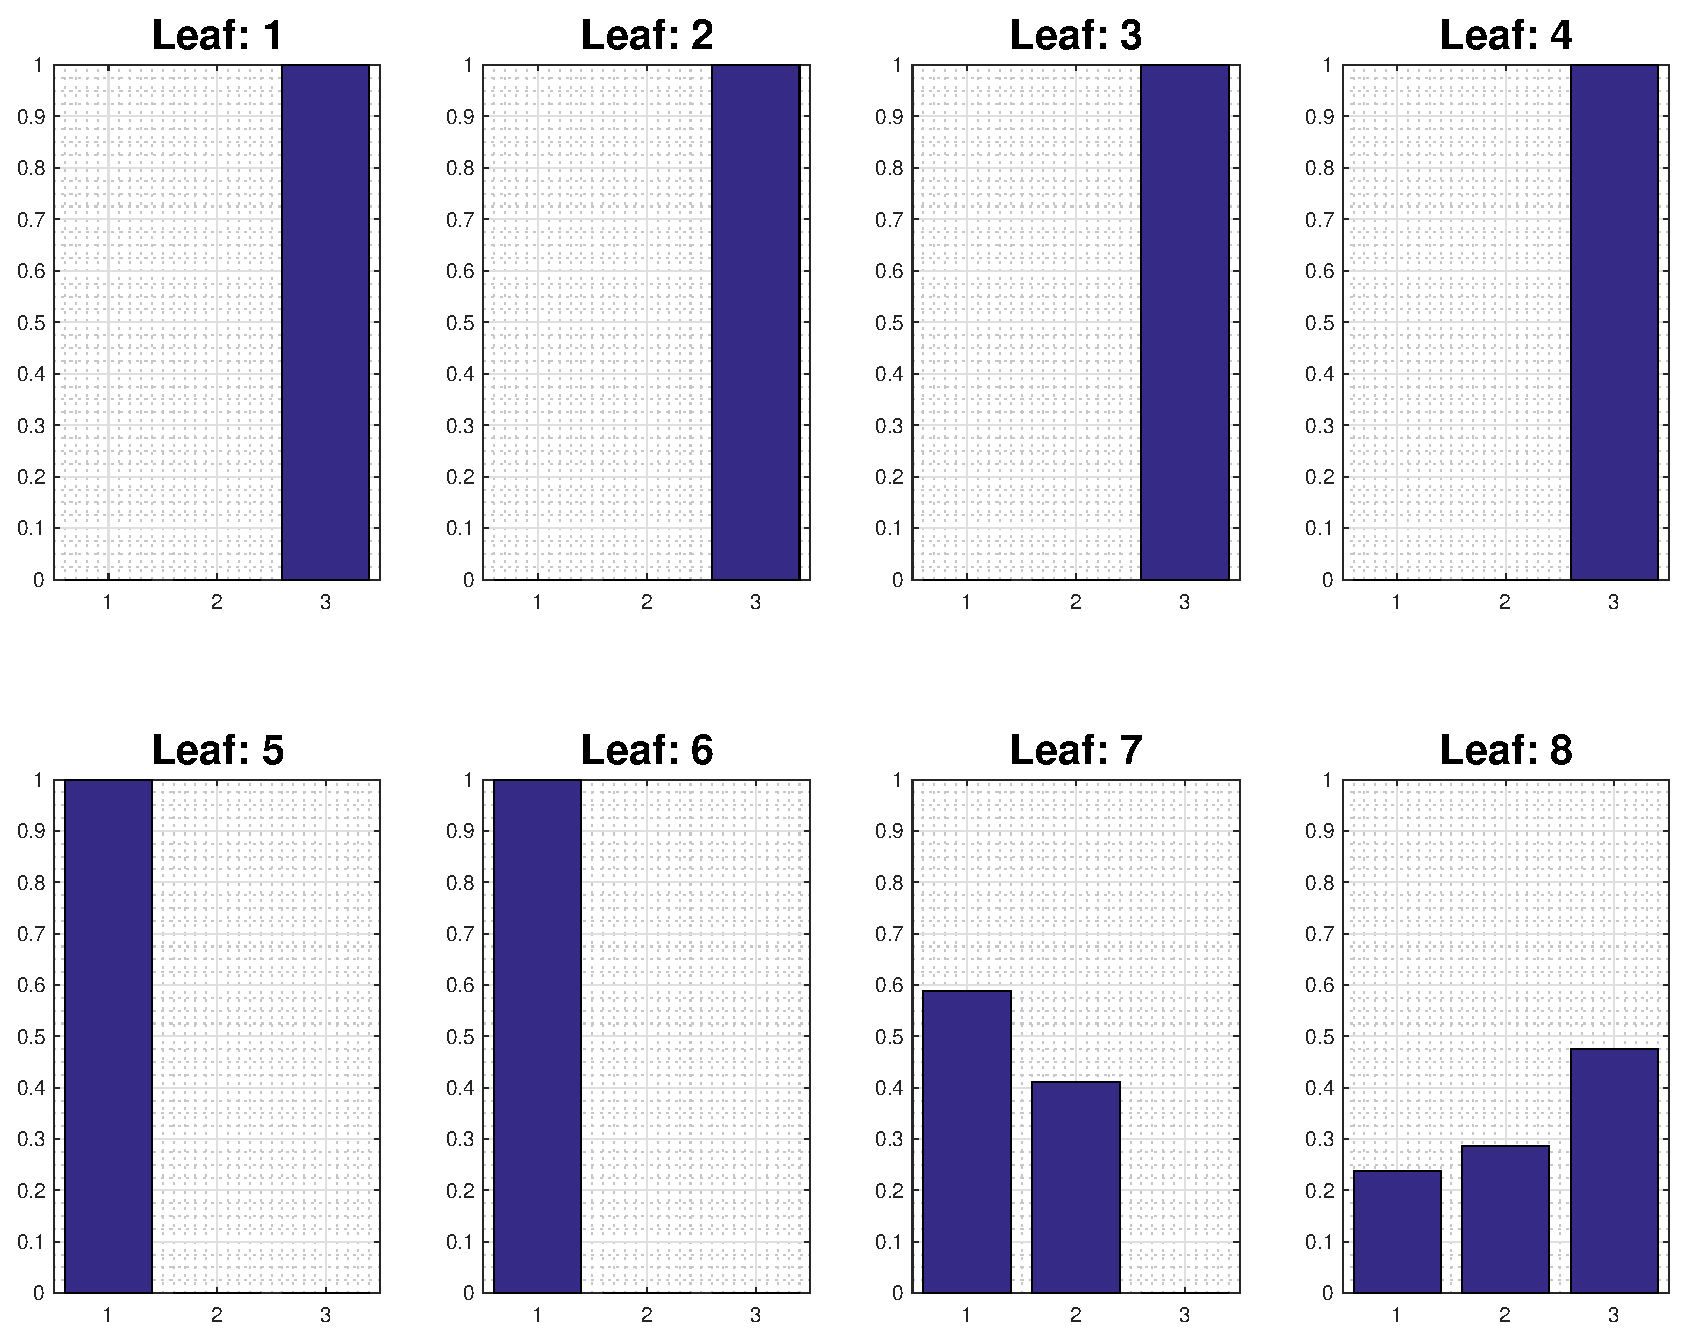
\includegraphics[width=\columnwidth]{leaf_node_distributions}
    \caption{Overview of spectral subtraction process}
    \label{fig:spec_sub_overview}
\end{figure}


\end{document}